\documentclass{beamer}

\usepackage[frenchb]{babel}
\usepackage[utf8]{inputenc}

\usetheme{Frankfurt}

\title{Réalisation d'un outil de cartographie pour le progiciel \textit{Amplitude}}
\author{Romain ROUSSEAU}
\institute{Sopra Banking Software}
\date{\today}


\begin{document}
	
	\logo{
\includegraphics[height=1cm]{images/logoSopra}}
	
\begin{frame}[plain]
	\titlepage
\end{frame}

\AtBeginSection[]
{
\begin{frame}
	
	\tableofcontents[currentsection, hideallsubsections]
	
\end{frame} 
}

\logo{images/logoSopra}	


\begin{frame}[plain]
\frametitle{Introduction}

Stage du 9 avril au 31 août 2018.
\bigbreak
Cellule Architecture de \textit{Sopra Banking Software} à Tours.

\end{frame}


\begin{frame}

\frametitle{Sommaire}

\tableofcontents

\end{frame}

\section{Présentation de l'entreprise}

\begin{frame}
\frametitle{Le groupe \textit{Sopra Steria}}

\begin{block}{Deux entités distinctes:}
	\begin{description}
		\item[Sopra] : créée en 1968, développement de logiciels dans le domaine bancaire et de la RH
		\item[Steria] : créée en 1969, SSII travaillant dans le secteur public
	\end{description}
\end{block}

\bigbreak 

Fusion des deux structures en 2015 pour former le groupe \textit{Sopra Steria}.

\bigbreak

Chiffre d'affaire de 3,8 milliard d'euros en 2017.

\end{frame}

\begin{frame}
\frametitle{\textit{Sopra Banking Software}}

Filiale du groupe \textit{Sopra Steria} créée en 2012 suite à de nombreux rachats de société (dont le groupe \textit{Delta Informatique}).

\bigbreak

Fournisseur de solutions globales : progiciels bancaires, services d'intégration, support, conseil... 

\bigbreak

800 banques dans 70 pays (Europe, Afrique et Moyen-Orient principalement)

\end{frame}

\begin{frame}
\frametitle{Le progiciel \textit{Amplitude}}

\textit{Amplitude}, solution de \textit{core banking} proposée pour traiter de manière intégrée toutes les problématiques bancaires.

\bigbreak

Première mise en production dans les années 90, initié par \textit{Delta Informatique}.

\bigbreak

Progiciel développé en langage Genero 4GL, aujourd'hui en version 11 (appelé \textit{Amplitude Up})

\end{frame}

\begin{frame}[plain]
\frametitle{Architecture d'\textit{Amplitude}}

\begin{center}
	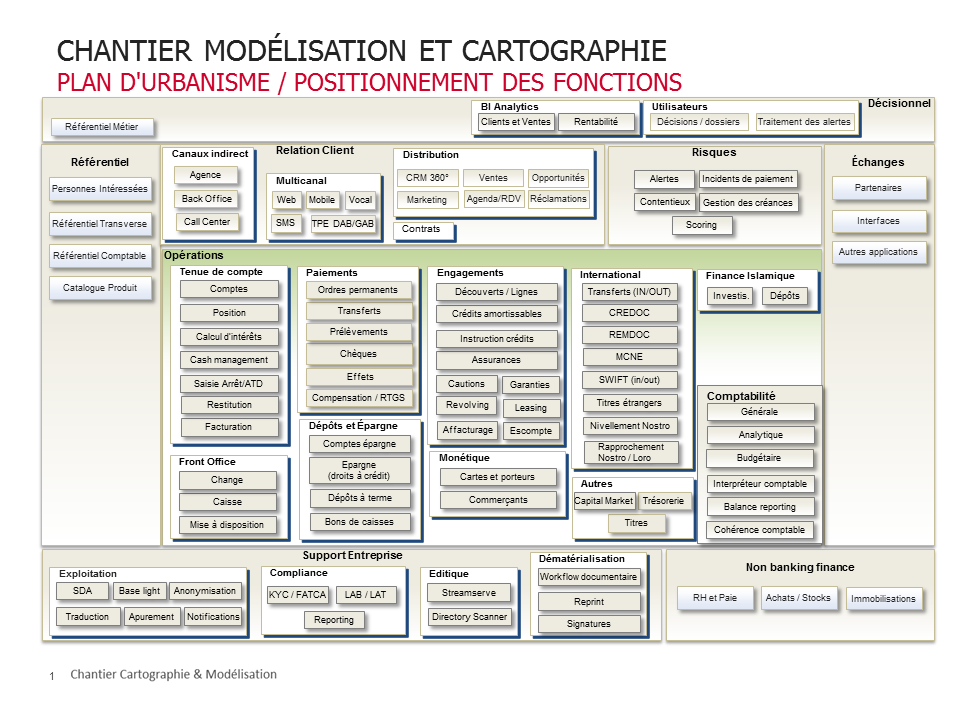
\includegraphics[width=11cm]{images/Cartographie_fonctionnelle}
\end{center}

\end{frame}

\begin{frame}
\frametitle{Arborescence d'\textit{Amplitude}}

\begin{description}
	\item[BaseProg] : liste des fichiers \textbf{BaseProg}. Ceux-ci répertorient les fichiers sources 4GL utilisés pour un programme donnée.
	\item[base\_ref] : schéma de référence \textit{Amplitude}, sert principalement à la compilation
	\item[bin] : liste des sources binaires
	\item[src] : répertoire sources 4gl et \textit{per} (les écrans) organisés par module
	\item[xcf] : liste des services métiers génériques (SMG) disponibles
\end{description}

\end{frame}

\section{Présentation du sujet}

\begin{frame}
\frametitle{Contexte du stage}

Demande effectuée par les architectes fonctionnels :

\begin{itemize}
	\item Maîtriser l’évolution du modèle de données \textit{Amplitude},
	\item Orienter l’analyste,
	\item Valider que les solutions proposées par l’analyste respectent bien les règles et principes d’architecture fonctionnelles et techniques du produit \textit{Amplitude}.
\end{itemize}

\end{frame}

\begin{frame}
\frametitle{Expressions des besoins}

\begin{itemize}
	\item Analyse et alerte sur les impacts développements
	\item Visualisation de la cartographie
\end{itemize}

\end{frame}

\begin{frame}
\frametitle{Déroulement du stage}

Tutoriels et mise à niveau (mois d'Avril)

\bigbreak

Modélisation de l'outil (mai jusqu'à début juin)

\bigbreak

Développement (de juin à août)

\end{frame}

\section{Technologies utilisées}

\begin{frame}
\frametitle{Spring Boot}

Framework facilitant la création d'application utilisant \textit{Spring} en automatisant ses configurations.

\begin{itemize}
	\item Proposer des solutions rapides et accessibles pour les développements \textit{Spring} ;
	\item Faciliter les configurations, même lorsque les paramètres souhaités diffèrent de ceux utilisés par défaut ;
	\item Proposer une panoplie d'options non-fonctionnelles (comme des serveurs embarqués \textit{Tomcat}, des options de sécurité, de mesures de performances, etc.).
\end{itemize}
\end{frame}

\begin{frame}
\frametitle{Spring Data}

Projet auxiliaire de \textit{Spring} permettant de faciliter l'accès aux données.

\bigbreak

Fonctionne avec tout type de base de données, relationnelle ou non.

\begin{block}{Spring Data REST}
Couche supérieure aux dépôts \textit{Spring Data} permettant d'exposer les données en REST.
\end{block} 

\end{frame}

\begin{frame}
\frametitle{Angular}

Framework open-source permettant de réaliser des applications Web.

\bigbreak 

Automatise certains procédés et permet de réaliser des animations complexes en peu de lignes de code.

\bigbreak

De nombreuses bibliothèques de styles existent : \textit{Bootstrap}, \textit{PrimeNG}, ...

\end{frame}

\section[Modélisation]{Modélisation de l'outil}

\begin{frame}
\frametitle{Modélisation de l'outil}

Partie back-end (gestion des données, alimentation de la base) avec Spring Boot et Spring Data. 

\bigbreak

Partie front-end (visualisation des données) avec Angular.

\bigbreak

Structure MVVM (Modèle - Vue - Vue/Modèle)

\end{frame}

\begin{frame}
\frametitle{Modélisation de l'outil}

La cartographie sera séparée en deux parties:

\begin{itemize}
	\item Cartographie fonctionnelle (domaines, fonctions, sous-fonctions, ...) lié à une base de données existante
	\item Cartographie technique (programmes, fichiers 4GL, ...) géré par notre alimentation et notre propre base de données
\end{itemize}

\end{frame}

\begin{frame}
\frametitle{Chiffrage}

Après la réalisation du chiffrage du développement, les temps vont être estimés trop courts pour la finalisation de l'outil.

\bigbreak

L'objectif sera de terminer la partie back-end avant la fin de mon stage.

\end{frame}

\section[Développement]{Éléments de Développement}

\begin{frame}
\frametitle{Exposition des données en REST}

\begin{center}
	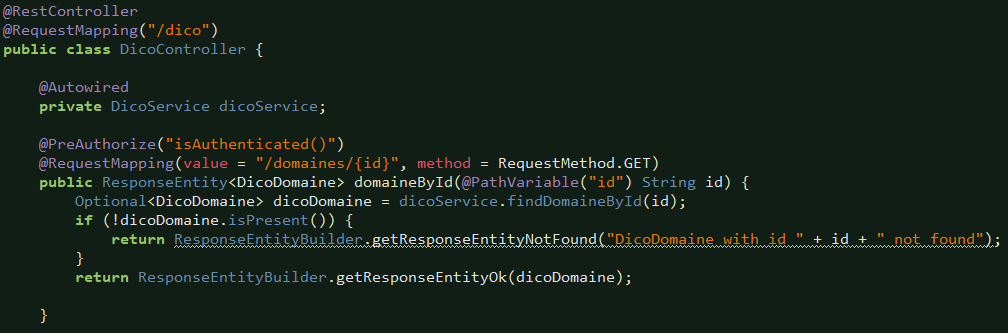
\includegraphics[width=11cm]{images/restController}
\end{center}

\end{frame}

\begin{frame}
\frametitle{Gestion du job d'alimentation des données}

Utilisation de \textit{Quartz} pour la gestion du job

\begin{itemize}
	\item Récupération des outils de développement d'\textit{Amplitude} via SVN
	\item Récupération des sources \textit{Amplitude}
	\item Création des programmes en base;
	\item Création des fichiers 4GL en base;
	\item Création des fonctions techniques;
	\item Association des programmes et des fichiers 4GL;
	\item Extraction du dictionnaire des programmes;
	\item Fonction de récupération des SMG.
\end{itemize}

\end{frame}

\begin{frame}
\frametitle{Aperçu de la page d'accueil}

\begin{center}
	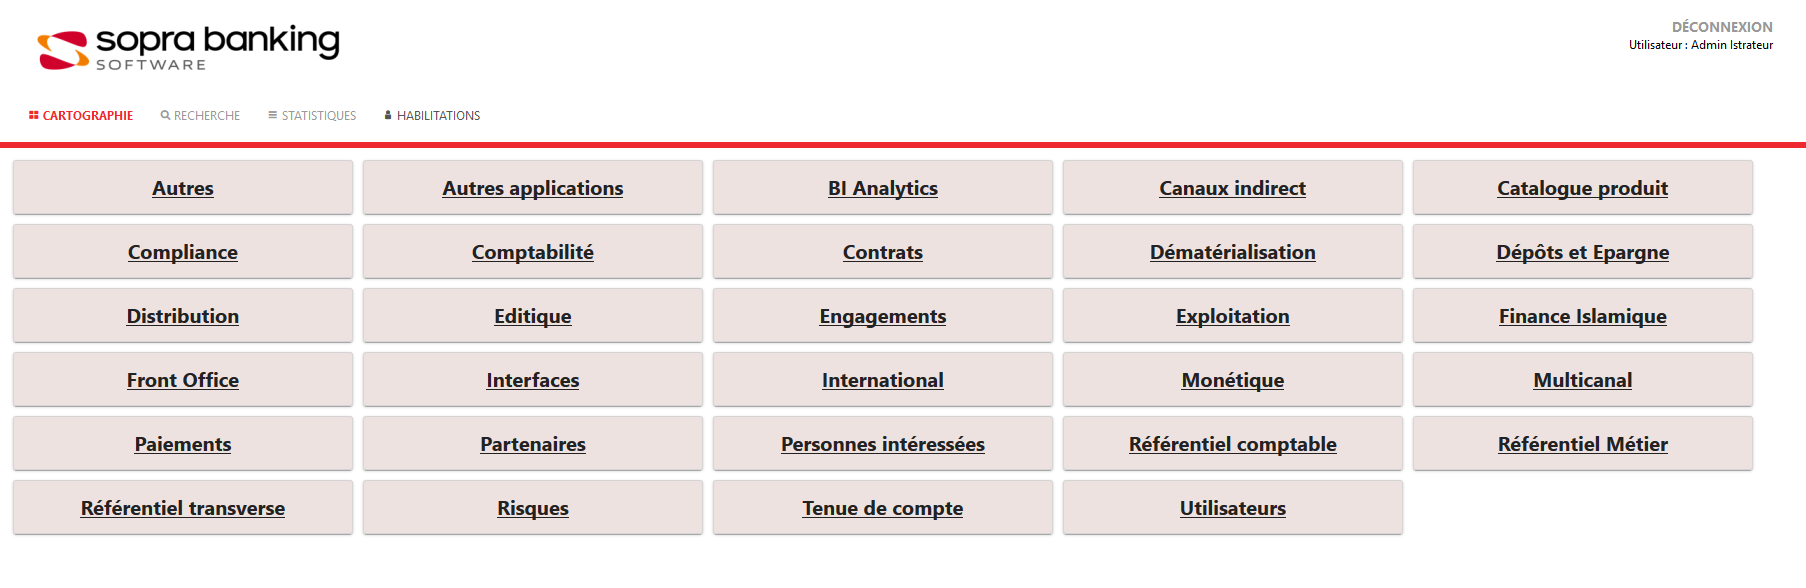
\includegraphics[width=11cm]{images/cartoAccueil}
\end{center}

\end{frame}


\section*{Bilan}

\begin{frame}
\frametitle{Bilan du stage}

La partie back-end est presque finalisée, les procédés d'alimentation de la base fonctionnent cependant les temps d'exécution sont trop longs pour le moment. 

\bigbreak

Sur un plan personnel, ce stage m'a permis d'acquérir énormément de compétences techniques.

\end{frame}

\begin{frame}
\frametitle{Remerciements}

Je tiens à remercier l'entreprise \textit{Sopra Banking Software} pour m'avoir accueilli, mon encadrant M. Alexandre DURAND pour sa confiance tout au long du stage et mes collègues sur place pour leur aide au quotidien.

\end{frame}

\end{document}